\documentclass[12pt]{article} 

\usepackage[latin1]{inputenc}
\usepackage[spanish]{babel}
\usepackage{color}
\usepackage{multicol}
\usepackage{amsmath}
\usepackage{amssymb}
\usepackage{enumerate}
\usepackage{graphics}
\usepackage{graphicx}

\title{PECAS}
\author{Sara Chica, Rodrigo Gualtero}
\date{20 de Octubre, 2012}

\begin{document}
\maketitle
\tableofcontents

\section{Introducci�n}
Este es un problema de la UVA, identificado con el c�digo \textit{10034}, en el cual Richie debe encontrar como conectar todas las pecas de la espalda de su padre con la menor distancia posible, para de esta forma reducir la cantidad de tinta que se usa para unirlas.

\begin{center}
	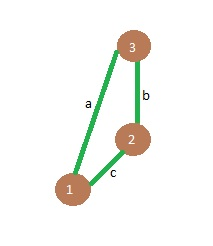
\includegraphics[width=0.50\textwidth]{Pecas.jpg}
	\\Ejemplo 1: 3 Pecas
\end{center}

En este ejemplo las pecas son \textit{1}, \textit{2} y \textit{3}; y las posibles conexiones son \textit{a}, \textit{b} y \textit{c}.
\\Utilizando algunas de estas 3 conexiones Richie debe poder conectar todas las pecas con la menor distancia.

\section{Definici�n del problema}
Para poder obtener la distancia entre peca y peca se hace necesario tomar cada peca como un punto ubicado en el plano cartesiano, por lo cual tendr�a componente \textit{x} y \textit{y}.

\begin{center}
	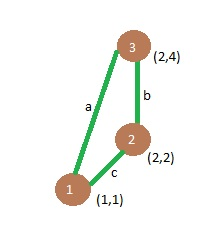
\includegraphics[width=0.50\textwidth]{PecasCarteciano.jpg}
	\\Ejemplo 2: 3 Pecas En plano cartesiano
\end{center}

En el \textit{ejemplo 2} se pueden observar las mismas 3 pecas que en el \textit{ejemplo 1}, pero ahora ubicadas en el plano cartesiano, cada una con sus respectivas cordenadas.

\subsection{Entrada}
Como primer lugar entra un valor que determina el n�mero de nodos, este debe ser entre 0 y 200.
\\Despu�s, separado por una linea en blanco, entra un n�mero, el cual indica la cantidad de pecas.
\\Finalmente entran todas las pecas con formato <<x y>>; donde \textit{x} y \textit{y} pueden ser n�meros reales.
\subsection{Salida}
Imprime la distancia m�s corta para conectar todas las pecas.

\section{Modelamiento matem�tico}
Sea G un grafo, $G(V,L)$, donde
\\
\\V es el conjunto de nodos del grafo, 
\[ V=\left\{ a_{1}, a_{2}, ... , a_{n} \right\}  \]
\\y L es el conjunto de todas las conexiones, 
\[ L= \left\{(a_{1},a_{2}),(a_{1},a_{3}), ... , (a_{1},a_{n}), (a_{2},a_{3}), (a_{2},a_{4}), ... , (a_{n-1},a_{n})\right\} \]
\\Este grafo cumple con las siguientes propiedades:
\begin{enumerate}
	\item El grafo es conexo, es decir existe una sucesi�n de arcos tal que es posible encontrar un camino para llegar a cualquier elemento del 		Conjunto.
	\item El grafo es no dirigido, es decir $(a,b)=(b,a)$.
  \item Ningun nodo tiene conexi�n consigo mismo, es decir no existe una conexi�n tal que $(a,a)$; es decir $(a,a) \notin L$
\end{enumerate}

\section{Planteamiento de la Soluci�n}
Para solucionar el problema se debe usar un algoritmo que permita encontrar el camino m�s corto entre dos nodos, para ello existen ya algunos, como lo son:
\begin{enumerate}
	\item Algoritmo de Dijkstra: Encuentra el camino m�s corto desde un �nico nodo origen, hasta todos los otros del grafo.
	\item Algoritmo de Bellman-Ford: Encuentra el camino m�s corto desde un nodo origen, permitiendo que el peso de alg�n arco sea negativo.
	\item Algoritmo de Floyd-Warshall: Encuentra el camino m�s corto entre todos los nodos del grafo.
	\item Algoritmo de Kruskal: Encuentra el camino m�s corto el cual pueda conectar todos los nodos, sin necesidad de tener un nodo origen.
\end{enumerate}

Por las caracter�sticas del problema se hace m�s conveniente utilizar el algoritmo de Kruskal.
\\Lo que hace este algoritmo como primera medida es organizar el arreglo de acuerdo a los pesos que tenga cada arco; luego de esto comienza a mirar las diferentes conexiones para hallar el camino m�s corto por medio del cual se puedan conectar todos los nodos. 

\section{Conclusiones}
\begin{enumerate}
	\item Entre los algoritmos consultados el que permite resolver el problema de una forma m�s eficiente es el de Kruskal, ya que, como primera medida no necesita un nodo de origen, y adem�s de esto, est� hecho para resolver problemas de este tipo.
	\item Existen varias implementaciones del algoritmo, por lo cual es importante cerciorarse si el algoritmo implementa el ordenamiento del arreglo, en caso de que no, se hace necesario pasarle este ordenado de peso menor a mayor.
	\item Estos algoritmos que resuelven problemas en donde se debe encontrar el camino m�s corto, tienen aplicaciones en redes y telecomunicaciones, facilitan el dise�o de sistemas, entre otros.
\end{enumerate}
\end{document}